\documentclass[tikz,border=10pt]{standalone}
\usepackage{amsmath,amssymb}
\usepackage{newpxtext,newpxmath}
\usetikzlibrary{arrows.meta,decorations.markings,calc,backgrounds}

\definecolor{inkDark}{HTML}{1E293B}
\definecolor{slateSub}{HTML}{334155}
\definecolor{pathBlue}{HTML}{005A9C}
\definecolor{accentRed}{HTML}{B91C1C}
\definecolor{accentTeal}{HTML}{0E6251}
\definecolor{accentAmber}{HTML}{B45309}
\definecolor{bandBlue}{HTML}{DBEAFE}
\definecolor{boxFill}{HTML}{F8FAFC}

\begin{document}
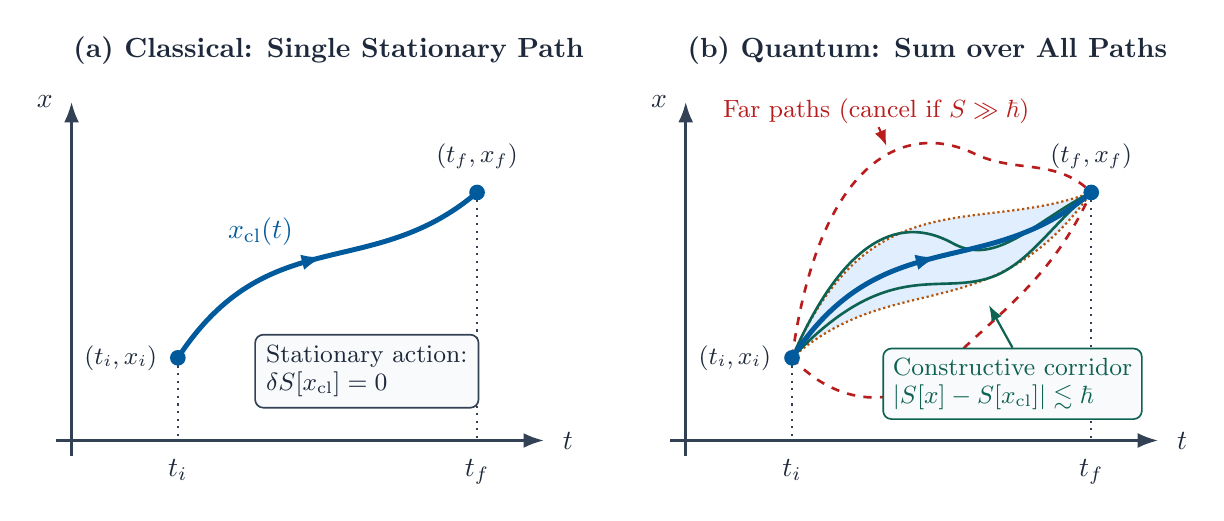
\begin{tikzpicture}[
    >=Latex,
    every node/.style={font=\normalsize, text=inkDark},
    axis/.style={-{Latex[length=2.6mm,width=1.9mm]}, line width=0.95pt, draw=slateSub},
    clpath/.style={
        line width=1.8pt,
        draw=pathBlue,
        postaction={decorate},
        decoration={
            markings,
            mark=at position 0.52 with {\arrow{Latex[length=2.8mm,width=2.0mm]}}
        }
    },
    nearpath/.style={line width=0.95pt, draw=accentTeal},
    wildpath/.style={line width=0.95pt, draw=accentRed, dashed},
    pt/.style={circle, fill=inkDark, inner sep=2.0pt},
    paneltitle/.style={font=\bfseries\normalsize, text=inkDark, anchor=west},
    tagbox/.style={
        draw=slateSub, line width=0.6pt, rounded corners=3pt,
        fill=boxFill, inner sep=4pt, font=\small, text=inkDark
    }
]

    % =========================================================
    % Panel (a): Classical Mechanics
    % =========================================================
    \begin{scope}[shift={(0,0)}]
        \node[paneltitle] at (-0.1, 4.95) {(a) Classical: Single Stationary Path};

        % Axes
        \draw[axis] (-0.2, 0) -- (6.0, 0) node[right=3pt] {$t$};
        \draw[axis] (0, -0.2) -- (0, 4.3) node[left=3pt] {$x$};

        % Endpoints
        \coordinate (Ai) at (1.35, 1.05);
        \coordinate (Af) at (5.15, 3.15);

        % Dashed projection lines
        \draw[dotted, line width=0.75pt, draw=slateSub] (Ai) -- (1.35, 0) node[below=3pt] {$t_i$};
        \draw[dotted, line width=0.75pt, draw=slateSub] (Af) -- (5.15, 0) node[below=3pt] {$t_f$};

        % Classical trajectory
        \draw[clpath] (Ai) .. controls (2.5, 2.80) and (3.8, 2.00) .. (Af);

        % Endpoints & labels
        \node[pt, fill=pathBlue] at (Ai) {};
        \node[pt, fill=pathBlue] at (Af) {};
        \node[left=4pt, font=\small] at (Ai) {$(t_i, x_i)$};
        \node[above=5pt, font=\small] at (Af) {$(t_f, x_f)$};

        % Curve label
        \node[text=pathBlue, font=\normalsize\bfseries] at (2.40, 2.65) {$x_{\mathrm{cl}}(t)$};

        % Concise formula box in lower-right whitespace
        \node[tagbox, align=left] at (3.75, 0.88) {Stationary action:\\[-1pt] $\delta S[x_{\mathrm{cl}}] = 0$};
    \end{scope}

    % =========================================================
    % Panel (b): Quantum Mechanics (Sum over All Paths)
    % =========================================================
    \begin{scope}[shift={(7.8,0)}]
        \node[paneltitle] at (-0.1, 4.95) {(b) Quantum: Sum over All Paths};

        % Axes
        \draw[axis] (-0.2, 0) -- (6.0, 0) node[right=3pt] {$t$};
        \draw[axis] (0, -0.2) -- (0, 4.3) node[left=3pt] {$x$};

        % Endpoints
        \coordinate (Bi) at (1.35, 1.05);
        \coordinate (Bf) at (5.15, 3.15);

        % Dashed projection lines
        \draw[dotted, line width=0.75pt, draw=slateSub] (Bi) -- (1.35, 0) node[below=3pt] {$t_i$};
        \draw[dotted, line width=0.75pt, draw=slateSub] (Bf) -- (5.15, 0) node[below=3pt] {$t_f$};

        % Semiclassical constructive corridor around x_cl(t)
        \begin{scope}[on background layer]
            \fill[bandBlue, opacity=0.82]
                (Bi) .. controls (2.35, 3.35) and (3.70, 2.60) .. (Bf)
                     .. controls (3.90, 1.40) and (2.65, 2.20) .. (Bi) -- cycle;
            \draw[accentAmber, line width=0.8pt, densely dotted]
                (Bi) .. controls (2.35, 3.35) and (3.70, 2.60) .. (Bf);
            \draw[accentAmber, line width=0.8pt, densely dotted]
                (Bi) .. controls (2.65, 2.20) and (3.90, 1.40) .. (Bf);
        \end{scope}

        % Wild non-classical paths outside the corridor
        \draw[wildpath] (Bi) .. controls (1.70, 3.60) and (2.80, 4.05) .. (3.65, 3.65)
                             .. controls (4.20, 3.38) and (4.70, 3.60) .. (Bf);
        \draw[wildpath] (Bi) .. controls (1.90, 0.45) and (2.70, 0.35) .. (3.30, 0.95)
                             .. controls (4.00, 1.65) and (4.65, 2.05) .. (Bf);

        % Nearby paths inside the constructive corridor
        \draw[nearpath] (Bi) .. controls (2.15, 2.90) and (2.95, 2.75) .. (3.40, 2.50)
                             .. controls (3.95, 2.20) and (4.45, 2.80) .. (Bf);
        \draw[nearpath] (Bi) .. controls (2.60, 2.38) and (3.25, 1.80) .. (3.95, 2.10)
                             .. controls (4.40, 2.30) and (4.70, 2.80) .. (Bf);

        % Classical trajectory in center
        \draw[clpath] (Bi) .. controls (2.5, 2.80) and (3.8, 2.00) .. (Bf);

        % Endpoints & labels
        \node[pt, fill=pathBlue] at (Bi) {};
        \node[pt, fill=pathBlue] at (Bf) {};
        \node[left=4pt, font=\small] at (Bi) {$(t_i, x_i)$};
        \node[above=5pt, font=\small] at (Bf) {$(t_f, x_f)$};

        % Clean annotations in whitespace
        \node[font=\small, text=accentRed, anchor=west] at (0.35, 4.18) {Far paths (cancel if $S \gg \hbar$)};
        \draw[-{Latex[length=2.0mm]}, draw=accentRed, line width=0.75pt] (2.45, 3.98) -- (2.55, 3.74);

        \node[
            draw=accentTeal, line width=0.6pt, rounded corners=3pt,
            fill=boxFill, inner sep=3.5pt, font=\small, text=accentTeal, align=left
        ] (tubelbl) at (4.15, 0.72)
            {Constructive corridor\\[-1pt] $|S[x]-S[x_{\mathrm{cl}}]| \lesssim \hbar$};
        \draw[-{Latex[length=2.0mm]}, draw=accentTeal, line width=0.8pt] (tubelbl.north) -- (3.85, 1.72);
    \end{scope}

\end{tikzpicture}
\end{document}
